\section{DSGVO: Datenschutz Grundverordnung}

\subsection{Wann DSGVO?}

Die DSGVO ist seit Ende Mai 2018 auch für Schweizer Unternehmen direkt
anwendbar, wenn:
\begin{itemize}
	\tightlist
	\item diese Waren oder Dienstleistungen in der EU/EWR anbieten
	(die Angabe des Preises in Euro genügt) und \textbf{dazu
	personenbezogene Daten} (z.B. Adressdaten, Kundenprofil) bearbeiten\\
	(Marktortprinzip: Art. 3 Abs. 2 DSGVO)
	\item diese das Verhalten von
	\textbf{Website-Besuchern aus der EU sammeln} und auswerten (Tracking
	durch Cookies, Profiling mit Tools wie Google Analytics, Facebook Pixel
	etc.)
	\item  diese regelmässig \textbf{Newsletter} an Empfänger in der EU
	versendet
	\item  diese im Auftrag oder als Konzernzentrale resp. -Mitglied
	eines in der EU domizilierten Unternehmens personenbezogene Daten
	bearbeiten
\end{itemize}

Zur Durchsetzung können die EU-Aufsichtsbehörden nun aber Auskünfte und
Überprüfungen veranlassen, Anweisungen erteilen sowie - bei wiederholter
schwerer Missachtung - Geldbussen bis zu € 10 resp. 20 Mio. oder bis zu 2\%
resp. 4\% des weltweit erzielten Jahresumsatzes verfügen. Die Massnahmen
müssen jeweils aber verhältnismässig und wirksam sein. „Bestrafung“ von
Unternehmen in der Schweiz noch unklar.

\mbox{}\\
Das DSGVO ist nur ein Mindeststandard um ein eruopäisch
vereinheitlichtes Datenschutzrecht zur Durchsetzung von mehrheitlich
bereits bestehenden Grundsätzen. Die einzelnen Mitgliedsstaaten können
weitergehende Regelungen erfassen.


\subsection{Rechte in der DSGVO}

\begin{itemize}
	\tightlist
	\item \textbf{Auskunftsrecht} und \textbf{Recht auf Datenübertragbarkeit}
	\item \textbf{Erweiterte Informationspflichten} gegenüber der betroffenen
	Person
	\item \textbf{Widerspruchsrecht}
	\item \textbf{Recht auf Löschung} (Recht auf Vergessen)
	\item Möglichkeit für \textbf{Abmahnungen} und Klagen von
	\textbf{Genugtuung} und \textbf{Schadenersatz} für die betroffene
	Person
	\item \textbf{Privacy by design} und \textbf{privacy by default} (!)
	\item Erweiterte \textbf{Dokumentationspflichten} (TOM's,
	Verarbeitungsverzeichnisse, Beweislastumkehr)
\end{itemize}


\subsubsection{TOM (Technische und organisatorische Massnahmen)}

Es muss dokumentiert werden, wie die informationstechnischen
Gerätschaften aufgestellt sind und wer verantwortlich ist.

\subsection{Was ist zu tun?}

\begin{figure}[H]
	\centering
	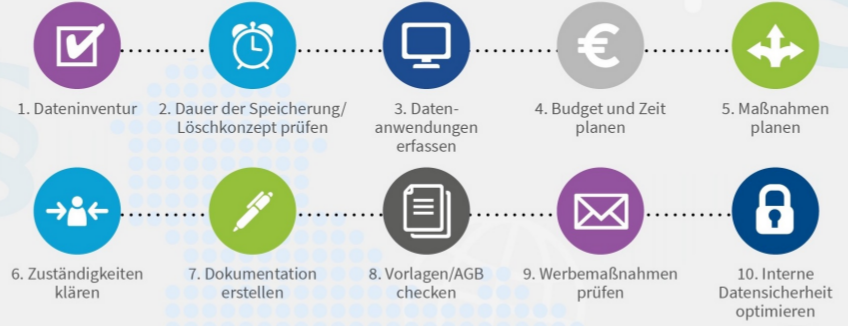
\includegraphics[width=.9\textwidth]{figures/dsgvoSteps.png}
	\caption{Schritte zur DSGVO-Konformität}
\end{figure}

\begin{itemize}
	\tightlist
	\item \textbf{Grundlage jedes Datenschutz-Audits ist die Erhebung des
	aktuellen Zustandes}:\\
	Welche personenbezogenen Daten sind vorhanden? In welcher Form und wo?
	Zu welchem Zweck? Wer zeichnet sich verantwortlich? Wer hat Zugang? Wie
	lange werden diese gespeichert? Handelt es sich um besonders
	schützenswerte Personendaten? Wie werden diese technisch \&
	organisatorisch geschützt? Wie wird das Risiko einer Verletzung \& deren
	Folgen beurteilt?
	\item Die DSGVO verlangt, dass bestehende Verträge (Einwilligungen),
	Datenschutzerklärungen (= Transparenz) und Abläufe angepasst werden. 
	Unternehmen	haben Rechenschaftspflichten (insb. TOMs und Verzeichnis der
	Verarbeitungstätigkeiten).
	\item Bestimmung und Angabe eines Datenschutzbeauftragten (= verantwortlich)
	sowie eines Vertreters in der EU! (= Anlaufstelle für Betroffene und 
	Aufsichtsbehörden für sämtliche	Datenschutzfragen).\\
	(Art. 27 DSGVO)
\end{itemize}

\subsection{DSGVO im Detail}
\begin{description}
	\tightlist
	\item[Ausbau der Rechte der betroffenen Personen] Aufklärungspflichten,
	Transparenz, Zweckbindung, ausdrückliche Einwilligung oder Bezug auf
	Rechtfertigungsgrund. (Art. 5/6 DSGVO).
	\item[Datenhaltung nur solange es der Zweck erfordert] Speicherbegrenzung
	(Art. 5 DSGVO)
	\item[Datenschutz durch Technikgestaltung] Privacy by Design
	(Art. 25 Abs. 1 DSGVO) und datenschutzfreundliche Voreinstellungen/Privacy
	by Default (Art. 25 Abs. 2 DSGVO).
	\item[Big Data] Pflicht zur vorgängigen Durchführung einer
	Datenschutz-Folgenabschätzung (Art. 35 DSGVO).
	\item[Meldepflichten bei Datenschutzverletzungen] an die zuständige
	Aufsichtsbehörde (Art. 33 DSGVO) sowie direkte Benachrichtigung der
	betroffenen Personen bei hohem Risiko von Persönlichkeitsverletzungen.
	\item[Benennung eines Datenschutzbeauftragten]  Bestimmung und Angabe eines
	Datenschutzbeauftragten (= verantwortlich) (Art. 37 DSGVO). Gegebenenfalls
	muss ein Vertreter des Unternehmens in der EU bestimmt werden
	(Art. 27 Abs. 1 DSGVO).
	\item[Auslagerung der Datenverarbeitung](Auftragsverarbeitung) nur auf der
	Grundlage eines Vertrages mit Standardvertragsklausel bei hinreichenden
	Garantien („Datenschutzsiegel“) des Auftragsdatenverarbeiters
	(Art. 28 Abs. 1 DSGVO).
	\item[Recht der betroffenen Person auf Datenübertragbarkeit] in
	strukturierter, maschinenlesbarer Form (Art. 20 DSGVO).
	\item[Keine Unter-Auftragsverarbeitung] (Sub-Sub-Akkordanten) ohne
	schriftliche Genehmigung des Verantwortlichen (Art. 28 Abs. 2 DSGVO).
\end{description}
